\documentclass[12pt]{amsart}
\usepackage{amsaddr}
\usepackage{marktext} 
%% Remove draft for real article, put twocolumn for two columns
\usepackage{svmacro}
\usepackage[utf8]{inputenc}
\usepackage{lineno}
\usepackage[style=alphabetic, backend=biber]{biblatex}
\addbibresource{bibliography.bib}

%% commentary bubble
\newcommand{\SV}[2][]{\sidenote[colback=green!10]{\textbf{SV\xspace #1:} #2}}

%% Title 
\title{ MATH 104: Homework 4}
\author{Due date: In class -- Wednesday, March 13, 2024}
\address{Fulbright University, Ho Chi Minh City, Vietnam}

%\author{Co-author}
%\address{  }
%\email {  }
%
\date{\today}

\begin{document}

\maketitle
\begin{problem}
Find an equation of the tangent plane to the given surface at the specified point.

\begin{enumerate}
    \item $z=2 x^2+y^2-5 y,(1,2,-4)$
    \item $z=e^{x-y}, \quad(2,2,1)$
    \item   $z=x / y^2,(-4,2,-1)$
    \item   $z=x \sin (x+y), \quad(-1,1,0)$
    \item   $z=\ln (x-2 y), \quad(3,1,0)$
\end{enumerate}
\end{problem}

\begin{problem}
    Verify the linear approximation at $(0,0)$ of the following
    \begin{enumerate}
        \item $e^x \cos(xy) \approx x + 1 $
        \item $\frac{y-1}{x+1} \approx x + y - 1 $
    \end{enumerate}
\end{problem}

\newpage

\begin{problem}
The wave heights $h$ in the open sea depend on the speed $v$ of the wind and the length of time $t$ that the wind has been blowing at that specd. Values of the function $h=f(v, t)$ arc recorded in feet in the following table. Use the table to find a linear approximation to the wave height function when $v$ is near 40 knots and $t$ is near 20 hours. Then estimate the wave heights when the wind has been blowing for 24 hours at 43 knots.

\begin{figure}[h!]
    \begin{center}
        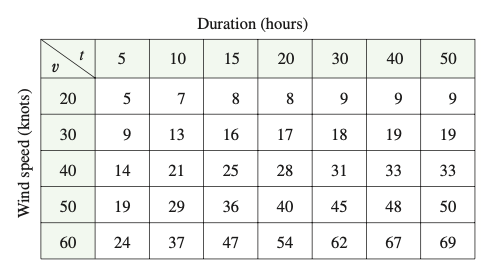
\includegraphics[width=0.7\textwidth]{wind}
    \end{center}
\end{figure}

\end{problem}

\begin{problem}
    If $R$ is the total resistance of three resistors, connected in parallel, with resistances $R_1, R_2, R_3$, then
$$
\frac{1}{R}=\frac{1}{R_1}+\frac{1}{R_2}+\frac{1}{R_3}
$$

If the resistances are measured in ohms as $R_1=25 \Omega$, $R_3=40 \Omega$, and $R_3=50 \Omega$, with a possible error of $0.5 \%$ in each case, estimate the maximum error in the calculated value of $R$.
\end{problem}

\end{document}
